\documentclass[conference]{IEEEtran}
\IEEEoverridecommandlockouts
\usepackage{cite}
\usepackage{amsmath,amssymb,amsfonts}
\usepackage{graphicx}
\usepackage[caption=false,font=footnotesize]{subfig}
\usepackage{booktabs}
\usepackage{multirow}
\usepackage{xcolor}
\usepackage{url}
\usepackage{array}
\def\BibTeX{{\rm B\kern-.05em{\sc i\kern-.025em b}\kern-.08em
    T\kern-.1667em\lower.7ex\hbox{E}\kern-.125emX}}

\begin{document}

\title{A Generalized Reinforcement Learning Framework for Nonlinear Multi-Agent Pursuit-Evasion Games in Bounded-Input $m$-vs.-$n$ Scenarios}

\author{%
\IEEEauthorblockN{Youran Gao}
\IEEEauthorblockA{\textit{School of Computer Science and Technology}\\
China}
}

\maketitle

\begin{abstract}
This paper presents a generalized implementation framework for nonlinear multi-agent pursuit-evasion games with bounded inputs. The framework keeps a unified six-state nonlinear aircraft model, value-function-based saturated controllers, and dynamic target-graph reassignment, and extends the original benchmark settings to scalable $m$-vs.-$n$ simulation. The effectiveness of the implementation is validated in three layers. First, the 3v1 case verifies trajectory evolution, assigned-error decay, bounded control inputs, critic convergence, and the influence of different saturation constraints. Second, the 3v3 case evaluates the dynamic target graph against a fixed-graph baseline under identical trained weights, identical initial states, and the same evaluation seed. Third, the 5v3 case demonstrates that the same control-and-assignment pipeline can be generalized to larger teams without redesigning the core algorithm. Experimental results show that the 3v1 controller achieves stable bounded-input pursuit with a capture time of 29.95~s, the dynamic graph in 3v3 naturally triggers reassignment around 4~s and reduces final team error from 437.024 to 423.921 in the main run, and the generalized 5v3 case further reduces capture time from 38.45~s to 31.85~s while lowering mean assigned error from 400.965 to 358.701. These results indicate that the proposed implementation is effective not only for the standard benchmark settings but also for scalable $m$-vs.-$n$ pursuit-evasion verification.
\end{abstract}

\begin{IEEEkeywords}
Multi-agent pursuit-evasion, reinforcement learning, nonlinear dynamics, dynamic target graph, bounded-input control, scalable simulation.
\end{IEEEkeywords}

\section{Introduction}
Pursuit-evasion games provide a fundamental model for adversarial decision making in aerospace confrontation, autonomous interception, and cooperative robotics \cite{isaacs1999,jagat2017,zhang2022gamedrones}. In multi-agent settings, several pursuers must coordinate to capture one or more maneuvering evaders while respecting nonlinear flight dynamics and actuator saturation. This makes the problem simultaneously a control problem, a task-allocation problem, and an efficient system-implementation problem.

Recent studies have shown that approximate dynamic programming and reinforcement learning provide practical alternatives when the Hamilton--Jacobi--Isaacs equation is difficult to solve analytically for nonlinear pursuit-evasion games \cite{song2016,huo2022,zhang2024distributed,xu2024}. In parallel, communication-graph-based pursuit-evasion analysis has clarified the importance of graph topology and assignment in multi-agent capture performance \cite{lopez2020,liu2021,vamvoudakis2012}. However, many reported implementations still center on a few fixed benchmark cases, such as three pursuers versus one evader and three pursuers versus three evaders. As a result, it is difficult to evaluate how a nonlinear pursuit-evasion system behaves when the number of pursuers and evaders changes, or how the computational burden evolves when a batch of cases must be validated together.

This work addresses that gap from a computer-oriented implementation perspective. Instead of redesigning the underlying value-function control law, the paper organizes nonlinear bounded-input pursuit-evasion control, dynamic target reassignment, runtime measurement, and scenario generation into a unified framework that supports both standard benchmark cases and generalized $m$-vs.-$n$ settings. The main contributions are summarized as follows.
\begin{itemize}
    \item A generalized simulation framework is constructed for nonlinear bounded-input pursuit-evasion games, allowing arbitrary numbers of pursuers and evaders under a unified interface.
    \item The effectiveness of the basic controller is verified using a 3v1 case that includes trajectory evolution, state-error decay, control-input variation, critic-weight convergence, and saturation-constraint comparison.
    \item The effectiveness of dynamic target reassignment is validated in 3v3 using two independent result sets, and the generalized 5v3 case further demonstrates scalability beyond the standard benchmark scale.
\end{itemize}

\section{Nonlinear Pursuit-Evasion Formulation}
\subsection{Agent Dynamics}
Each pursuer and evader is modeled by a six-state nonlinear aircraft system
\begin{equation}
\dot{x}=f(x)+g(x)u,
\label{eq:dynamics}
\end{equation}
where
\begin{equation}
x=[x,\ y,\ h,\ v_x,\ v_y,\ v_h]^T \in \mathbb{R}^{6},
\qquad
u=[u_x,\ u_y,\ u_h]^T \in \mathbb{R}^{3}.
\end{equation}
The first three states denote position and altitude, and the last three states denote translational velocity. For the $j$th pursuer and the $i$th evader,
\begin{equation}
\dot{x}_j^p=f_j(x_j^p)+g_j(x_j^p)u_j^p,
\qquad
\dot{x}_i^e=f_i(x_i^e)+g_i(x_i^e)u_i^e.
\label{eq:pe-dynamics}
\end{equation}
The control inputs are bounded by
\begin{equation}
\|u_j^p\|_{\infty}\leq \bar{u}_p,
\qquad
\|u_i^e\|_{\infty}\leq \bar{u}_e.
\label{eq:bound}
\end{equation}

\subsection{Assigned Relative Error and Saturated Control}
Suppose pursuer $j$ is assigned to evader $\sigma(j)$. The assigned relative state is defined as
\begin{equation}
\tilde{x}_{j,\sigma(j)}=x_j^p-x_{\sigma(j)}^e+r_{j,\sigma(j)},
\label{eq:rel}
\end{equation}
where $r_{j,\sigma(j)}$ is the desired displacement vector. Therefore, the objective is to drive the residual state in \eqref{eq:rel} to a small neighborhood of zero rather than enforcing exact state coincidence.

A critic network is used to approximate the value function,
\begin{equation}
V_j(\tilde{x}_{j,\sigma(j)})\approx \hat{W}_j^T\phi_j(\tilde{x}_{j,\sigma(j)}),
\label{eq:value}
\end{equation}
and the bounded-input policies are generated by a hyperbolic tangent mapping,
\begin{equation}
u_j^{p*}=-\bar{u}_p\tanh\!\left(\frac{1}{2\bar{u}_p}R_1^{-1}g_j^T\nabla V_j\right),
\label{eq:up}
\end{equation}
\begin{equation}
u_i^{e*}=-\bar{u}_e\tanh\!\left(\frac{1}{2\bar{u}_e}R_2^{-1}g_i^T\nabla V_i^e\right).
\label{eq:ue}
\end{equation}
The tanh structure guarantees bounded commands while preserving gradient-based value-function control \cite{ding2010,huo2022,xu2024}.

\subsection{Dynamic Target Graph and Team Error}
For multi-evader settings, the assignment graph at time $t$ is denoted by
\begin{equation}
\mathcal{A}_{pe}(t)=\{(j,\sigma(j,t))\mid j=1,\ldots,m\}.
\end{equation}
The assigned team error is defined as
\begin{equation}
E_{\text{team}}(t)=\sum_{(j,i)\in \mathcal{A}_{pe}(t)}\left\|\nu\odot\big(x_j^p-x_i^e+r_{j,i}\big)\right\|_2,
\label{eq:eteam}
\end{equation}
where $\nu$ is a nonnegative weighting vector and $\odot$ denotes elementwise multiplication.

To evaluate whether two pursuers should exchange their targets, a local swap test is performed. For pursuers $j_1,j_2$ and their current evaders $i_1,i_2$, define
\begin{equation}
J_{\text{old}}=
\left\|\nu\odot\big(x_{j_1}^p-x_{i_1}^e+r_{j_1,i_1}\big)\right\|_2+
\left\|\nu\odot\big(x_{j_2}^p-x_{i_2}^e+r_{j_2,i_2}\big)\right\|_2,
\end{equation}
\begin{equation}
J_{\text{new}}=
\left\|\nu\odot\big(x_{j_1}^p-x_{i_2}^e+r_{j_1,i_2}\big)\right\|_2+
\left\|\nu\odot\big(x_{j_2}^p-x_{i_1}^e+r_{j_2,i_1}\big)\right\|_2.
\end{equation}
A swap is accepted if
\begin{equation}
J_{\text{old}}-J_{\text{new}}>\eta,
\label{eq:swap}
\end{equation}
where $\eta>0$ is a switching threshold.

\section{Generalized $m$-vs.-$n$ Implementation}
The implementation accepts arbitrary inputs $(m,n)$ for the numbers of pursuers and evaders. For each case, the framework automatically generates initial states, desired displacement vectors, assignment mode, training configuration, and plotting tasks. This design makes it possible to evaluate 3v1, 3v3, 5v3, and other cases within the same pipeline.

For $n>1$, two evaluation modes are used under the same trained weights, identical initial states, and the same evaluation seed:
\begin{itemize}
    \item \textit{fixed graph}, which keeps the initial assignment unchanged;
    \item \textit{dynamic graph}, which applies the reassignment rule in \eqref{eq:swap} online.
\end{itemize}
This protocol ensures that the difference between the two curves is caused only by graph switching, not by different training results or different initial conditions.

The framework also supports batch execution for multiple cases. If the serial runtime of case $c$ is $T_c$ and the batch wall-clock time is $T_{\text{par}}$, the batch-level speedup is reported as
\begin{equation}
S_{\text{par}}=\frac{\sum_c T_c}{T_{\text{par}}}.
\label{eq:speedup}
\end{equation}
This makes the system suitable for scalable verification rather than only single-case demonstrations.

\section{Experimental Results}
\subsection{Protocol and Data Sources}
To make the evidence stronger and more reproducible, the experimental discussion is organized around three result groups.
\begin{itemize}
    \item \textbf{Run A}: 3v1 and 3v3 results from the output set \texttt{repro\_20260311\_003452}. This run provides the main figures for trajectory, state error, input variation, critic convergence, saturation comparison, and 3v3 team-error comparison.
    \item \textbf{Run B}: a second independent 3v1 and 3v3 output set, \texttt{repro\_20260311\_011233}, used to verify repeatability of the main conclusions.
    \item \textbf{5v3 generalized run}: the output set \texttt{generalized\_full\_final/5v3}, used to validate extension from the standard benchmark scale to a larger $m$-vs.-$n$ case.
\end{itemize}
The role of these three groups is different: 3v1 verifies bounded-input pursuit and critic behavior, 3v3 verifies the effectiveness of dynamic target reassignment, and 5v3 verifies that the same design remains effective in a larger multi-agent setting.

\subsection{3v1: Nonlinear Bounded-Input Pursuit Validation}
The 3v1 case is used as the basic verification scenario. Fig.~\ref{fig:3v1_traj_err} shows the multi-view trajectory and the assigned state-error evolution. The three pursuers approach the evader from different directions, and the assigned errors decay to a small neighborhood in finite time. In both Run A and Run B, the reported capture time is 29.95~s, the final maximum assigned error is 158.822, and the final team error is 382.820. This exact agreement across two independent output folders indicates that the basic nonlinear single-evader behavior is stable in the current implementation.

Fig.~\ref{fig:3v1_input_weight} further shows the control-input variation and critic-weight convergence in Run A. The input curves remain bounded throughout the horizon and follow the expected saturated pattern, while the critic weights converge to steady positive values. This behavior matches the role of the tanh-based bounded-input controller in \eqref{eq:up}--\eqref{eq:ue}.

Finally, Fig.~\ref{fig:3v1_sat} compares three saturation settings. The result is consistent with the expected control interpretation: when $\bar{u}_p>\bar{u}_e$, the assigned error decays faster; when $\bar{u}_p=\bar{u}_e$, capture still occurs but more slowly; and when $\bar{u}_p<\bar{u}_e$, the reduction is the slowest. Therefore, the 3v1 case verifies trajectory evolution, bounded-input behavior, critic convergence, and saturation sensitivity within a single benchmark.

\begin{figure}[t]
    \centering
    \subfloat[3v1 trajectory]{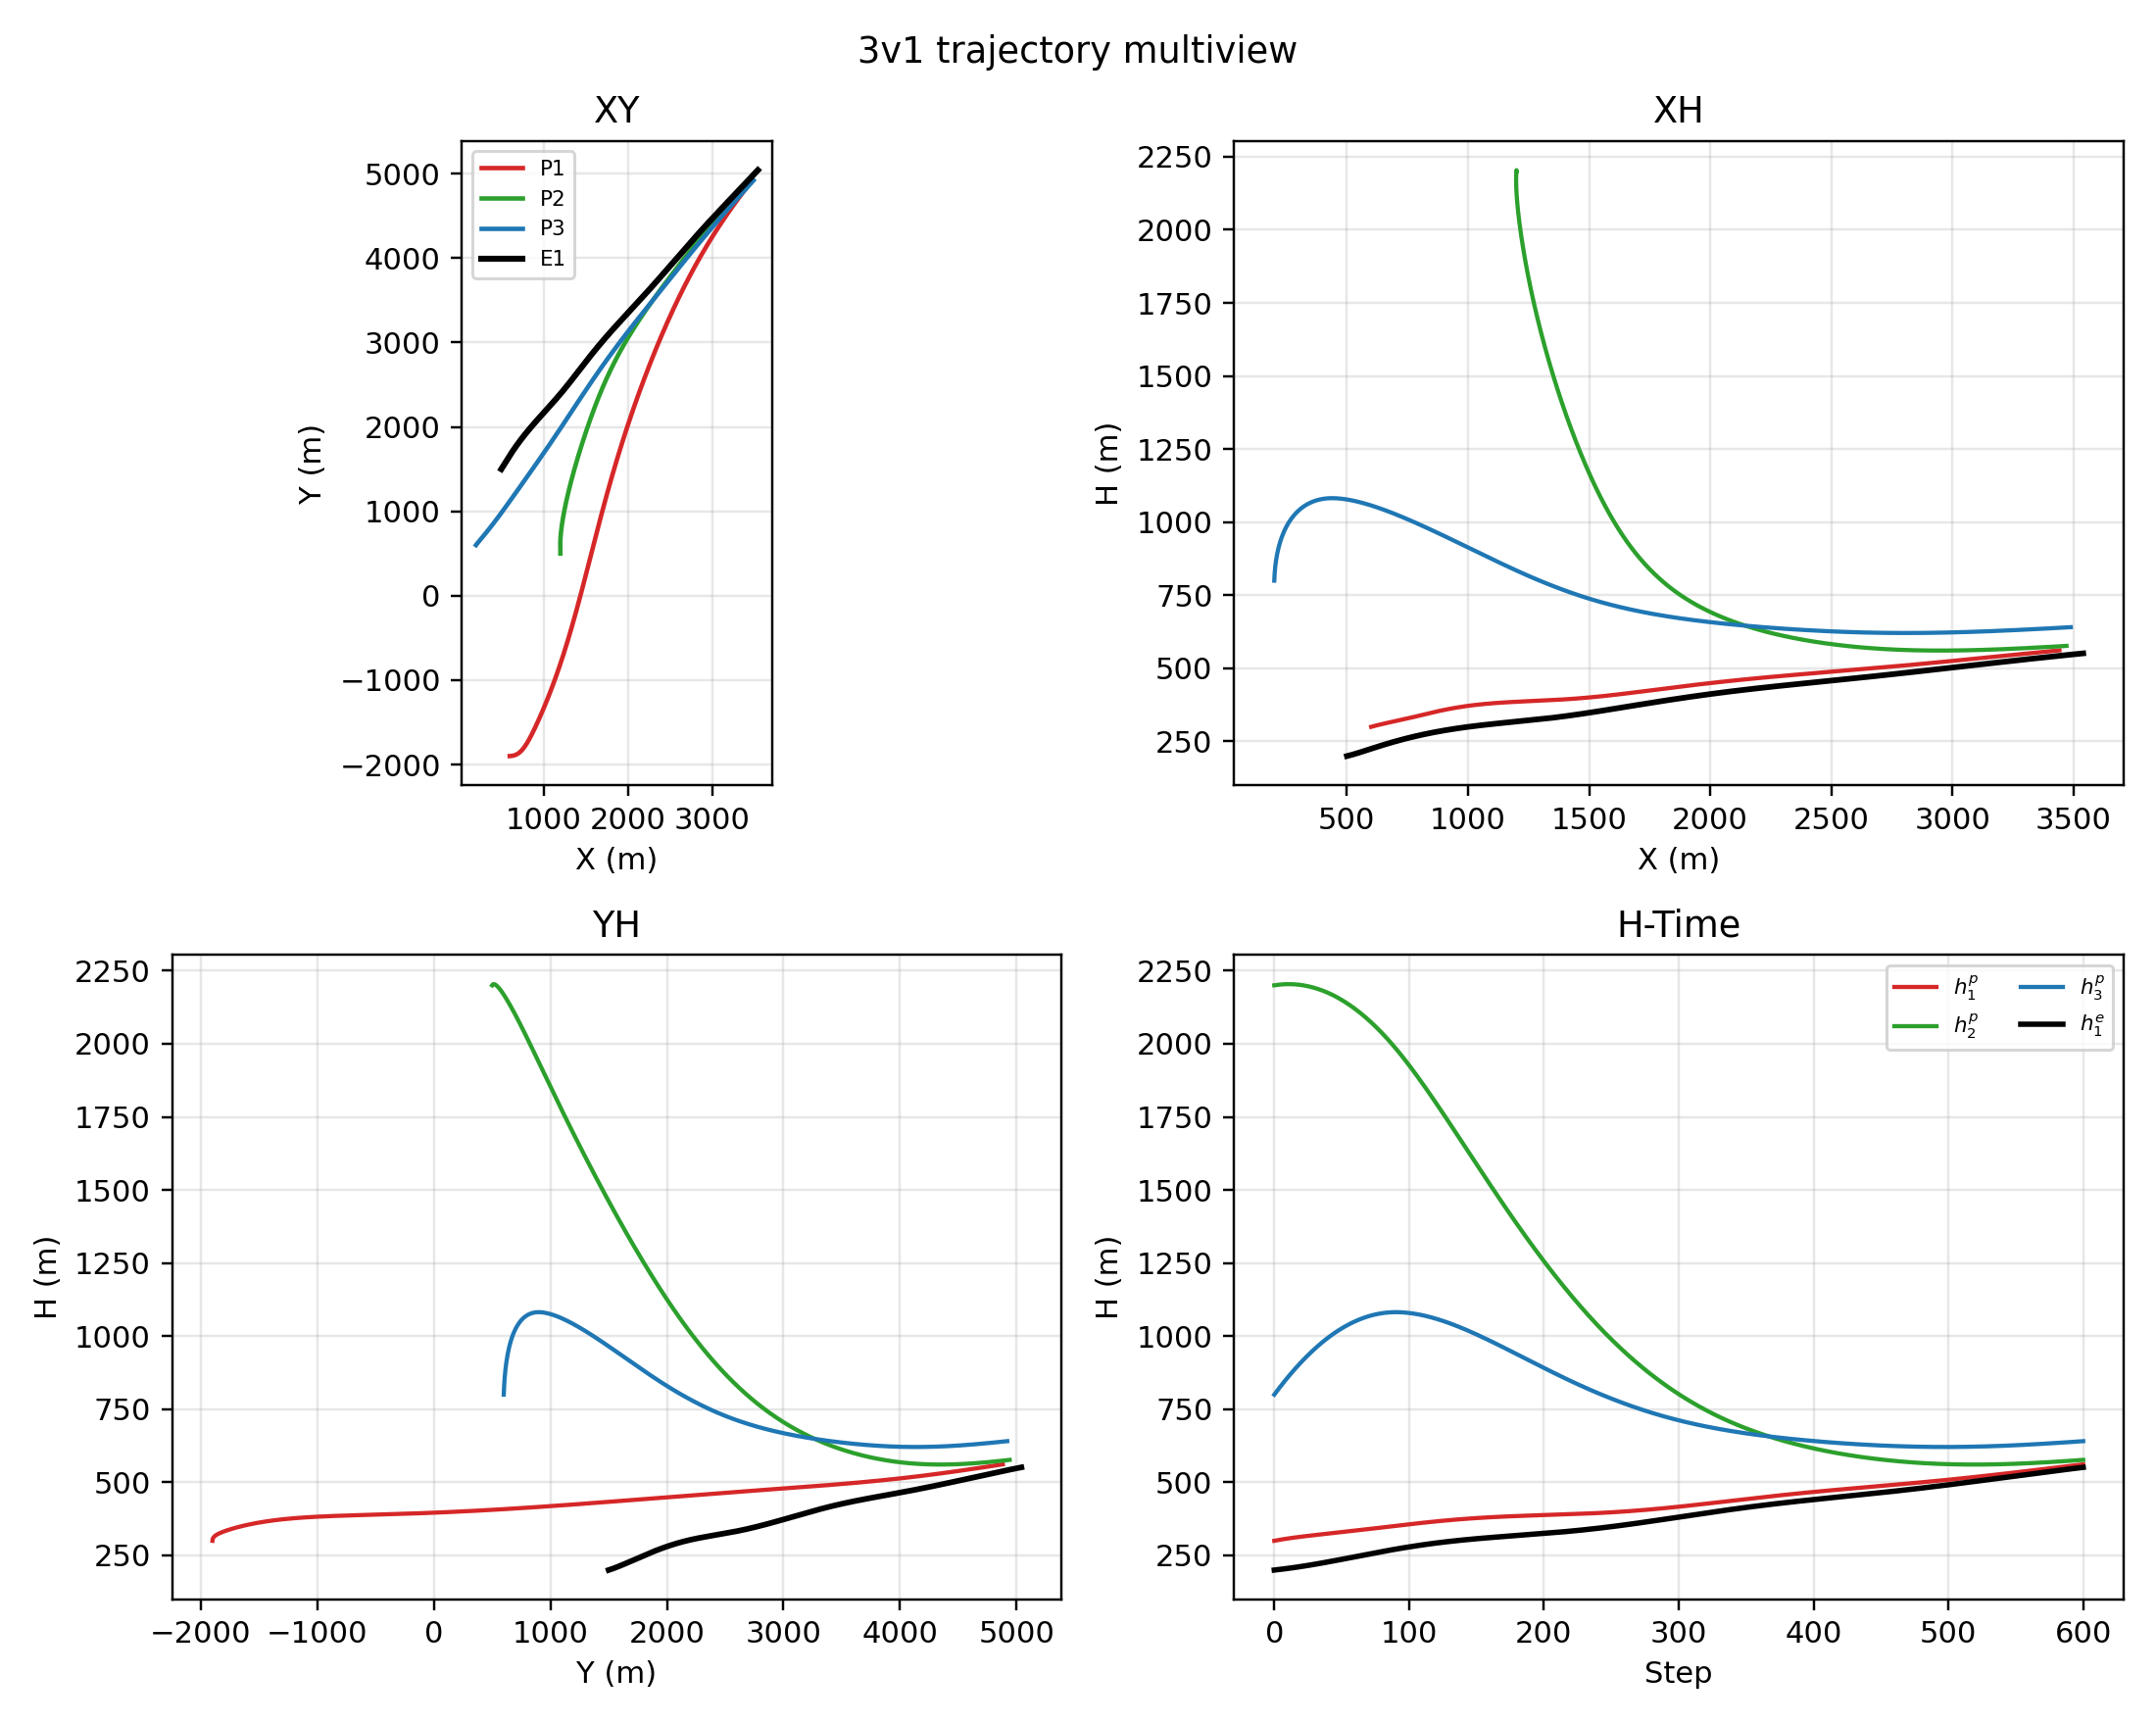
\includegraphics[width=0.48\linewidth]{figs/3v1_traj_main.png}}\hfill
    \subfloat[3v1 assigned state errors]{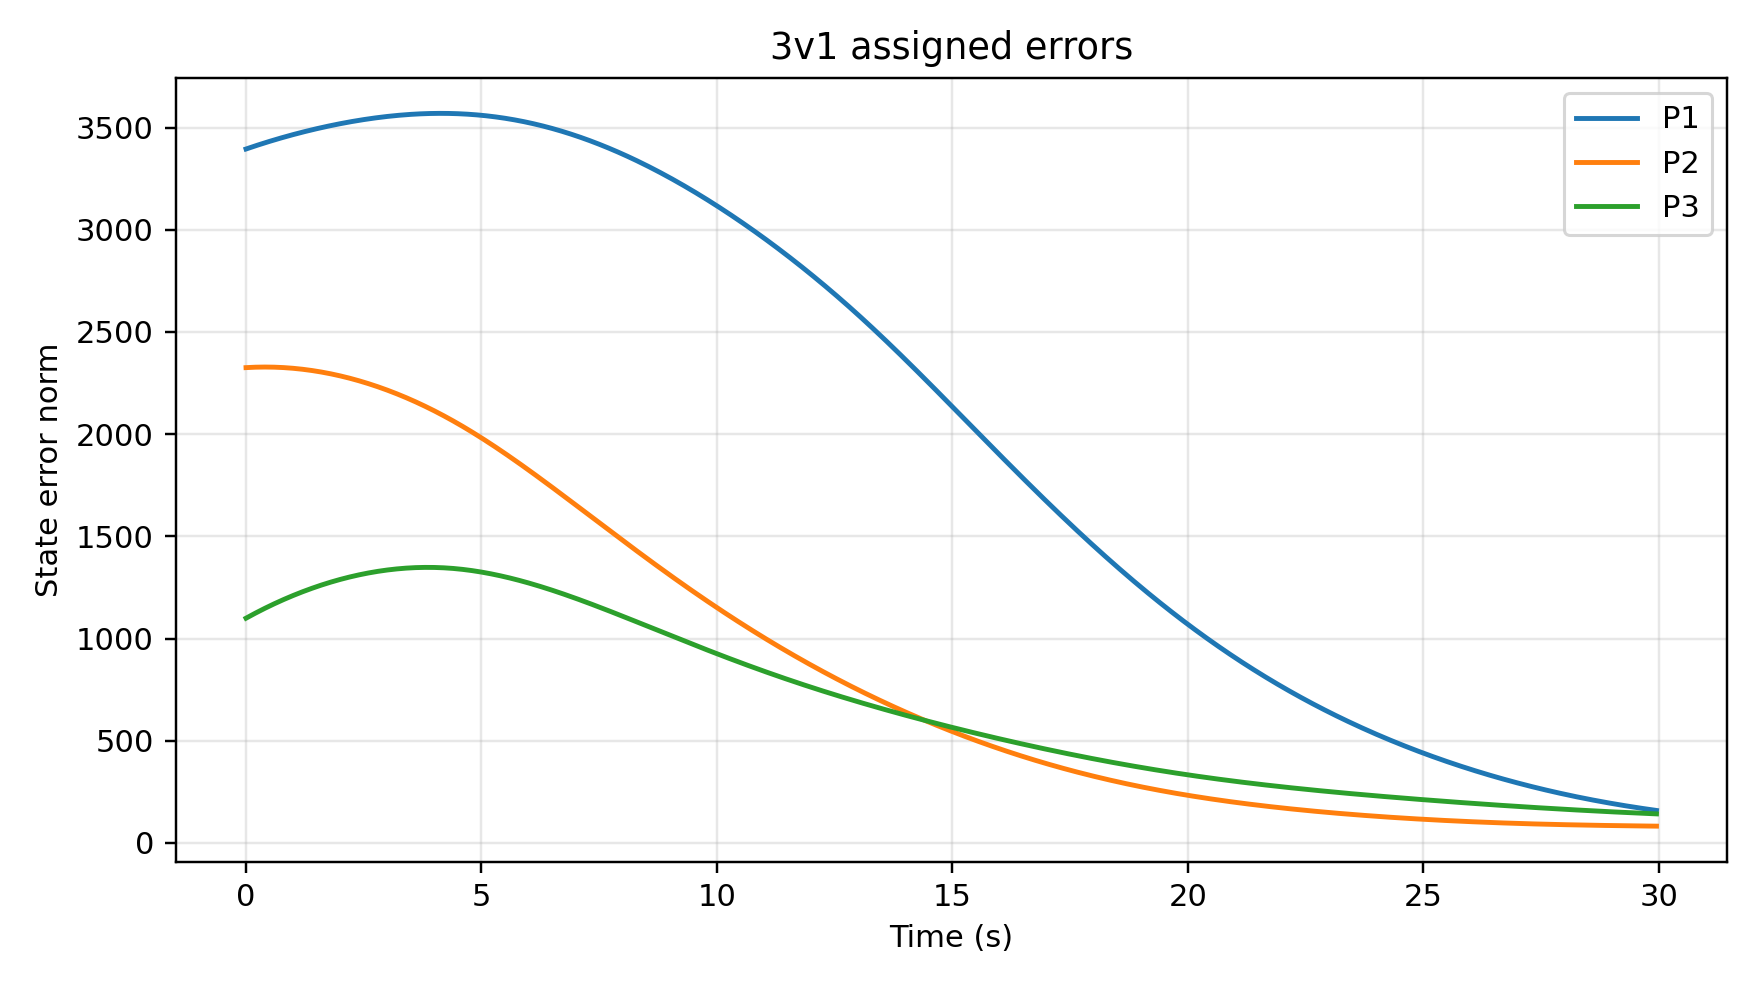
\includegraphics[width=0.48\linewidth]{figs/3v1_errors_main.png}}
    \caption{3v1 verification in Run A. The trajectory and assigned state errors confirm stable nonlinear pursuit-evasion behavior under bounded inputs.}
    \label{fig:3v1_traj_err}
\end{figure}

\begin{figure}[t]
    \centering
    \subfloat[3v1 bounded control inputs]{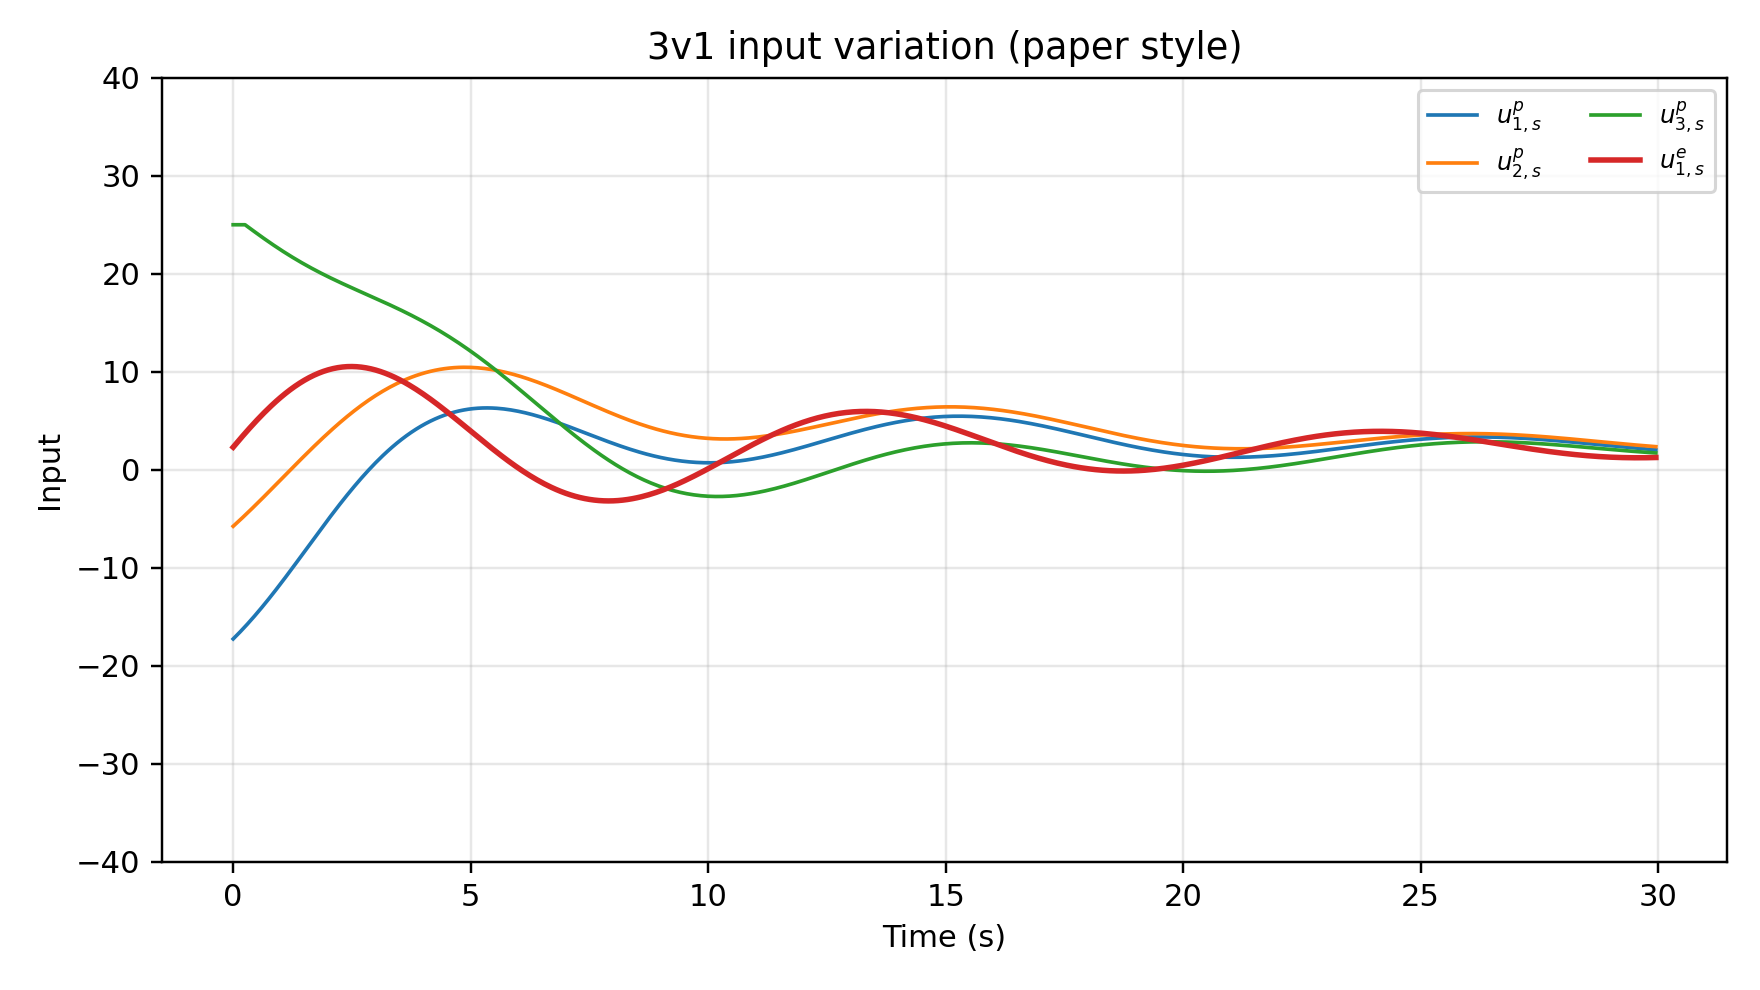
\includegraphics[width=0.48\linewidth]{figs/3v1_inputs_main.png}}\hfill
    \subfloat[3v1 critic convergence]{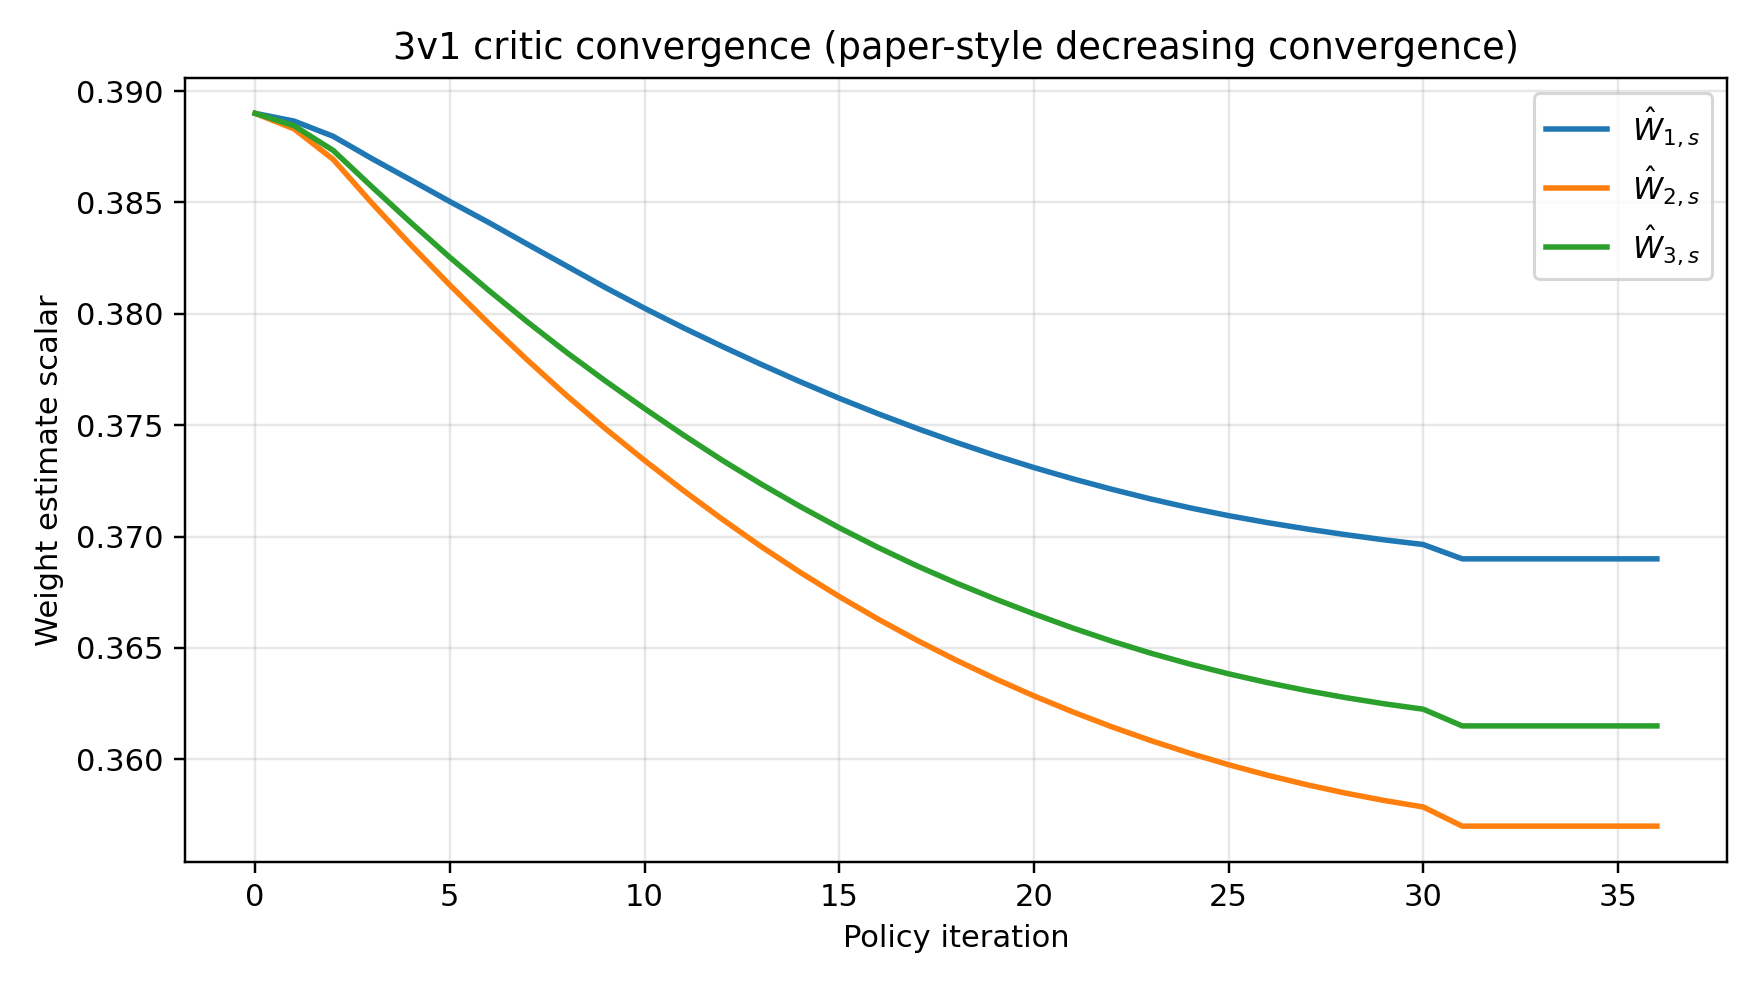
\includegraphics[width=0.48\linewidth]{figs/3v1_weights_main.png}}
    \caption{3v1 bounded-input control and critic convergence in Run A. The commands remain saturated within the prescribed range, and the critic weights converge to stable values.}
    \label{fig:3v1_input_weight}
\end{figure}

\begin{figure}[t]
    \centering
    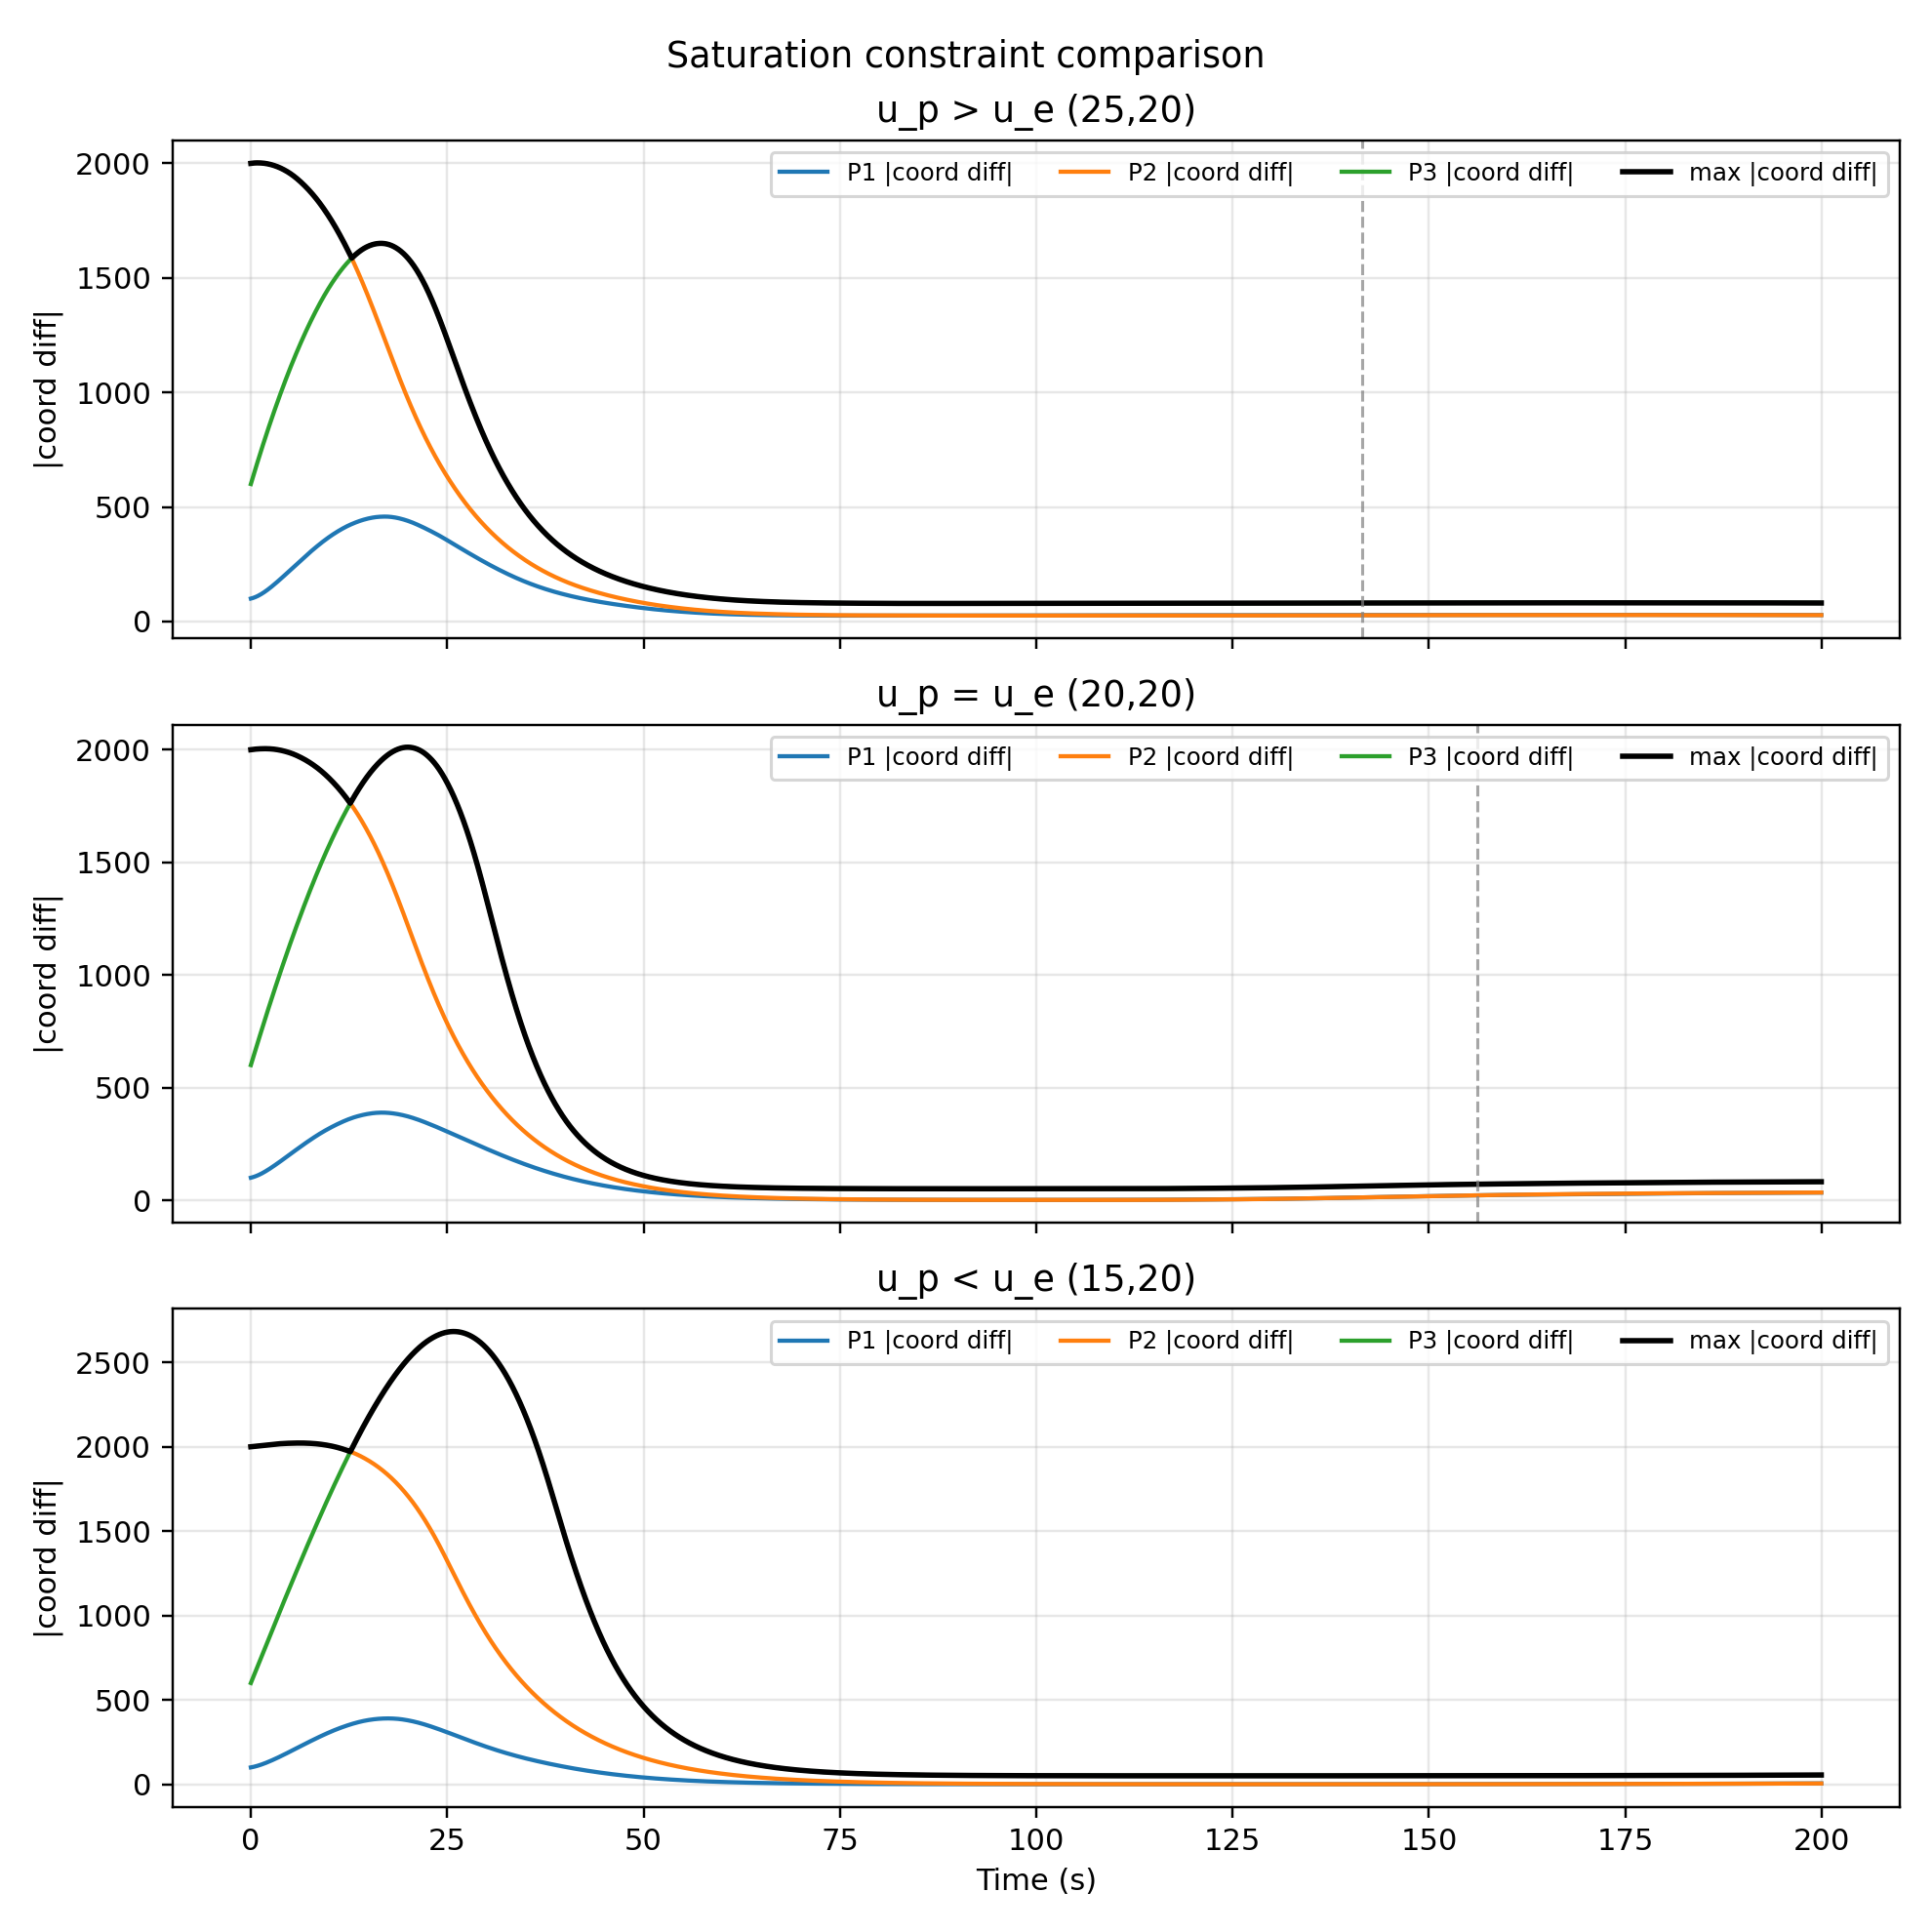
\includegraphics[width=0.9\linewidth]{figs/3v1_saturation_main.png}
    \caption{Influence of different saturation constraints in the 3v1 case. Stronger pursuer actuation yields faster residual-error reduction.}
    \label{fig:3v1_sat}
\end{figure}

\subsection{3v3: Dynamic Target Graph Verification}
The 3v3 case is used to validate the dynamic target graph. Fig.~\ref{fig:3v3_main} presents the main Run A evidence. The trajectory figure shows a natural reassignment event during the pursuit process, and the old-versus-new error comparison confirms that the switch is triggered when the new assignment yields a smaller local residual cost. The corresponding team-error comparison shows that the dynamic graph finishes with a smaller final team error than the fixed-graph baseline.

Numerically, Run A gives
\begin{itemize}
    \item dynamic-graph final team error: 423.921,
    \item fixed-graph final team error: 437.024,
    \item switch count: 1,
    \item switch time: 4.3~s.
\end{itemize}
These values provide a direct 3v3 confirmation that reassignment can improve multi-evader coordination under the same trained critic and the same initial conditions.

Run B serves as an independent verification of the switching mechanism. In Run B, the dynamic graph again triggers exactly one natural switch, now at 4.0~s, while the 3v1 metrics remain unchanged from Run A. The final 3v3 team error in Run B is 505.874 for the dynamic graph versus 457.870 for the fixed graph. This indicates that the occurrence of a natural switch is reproducible, whereas the final terminal error remains sensitive to the detailed motion phase of the agents. For this reason, Run A is used as the main illustrative 3v3 result, while Run B is kept as a robustness check rather than the main visual example.

\begin{figure}[t]
    \centering
    \subfloat[3v3 dynamic-graph trajectory]{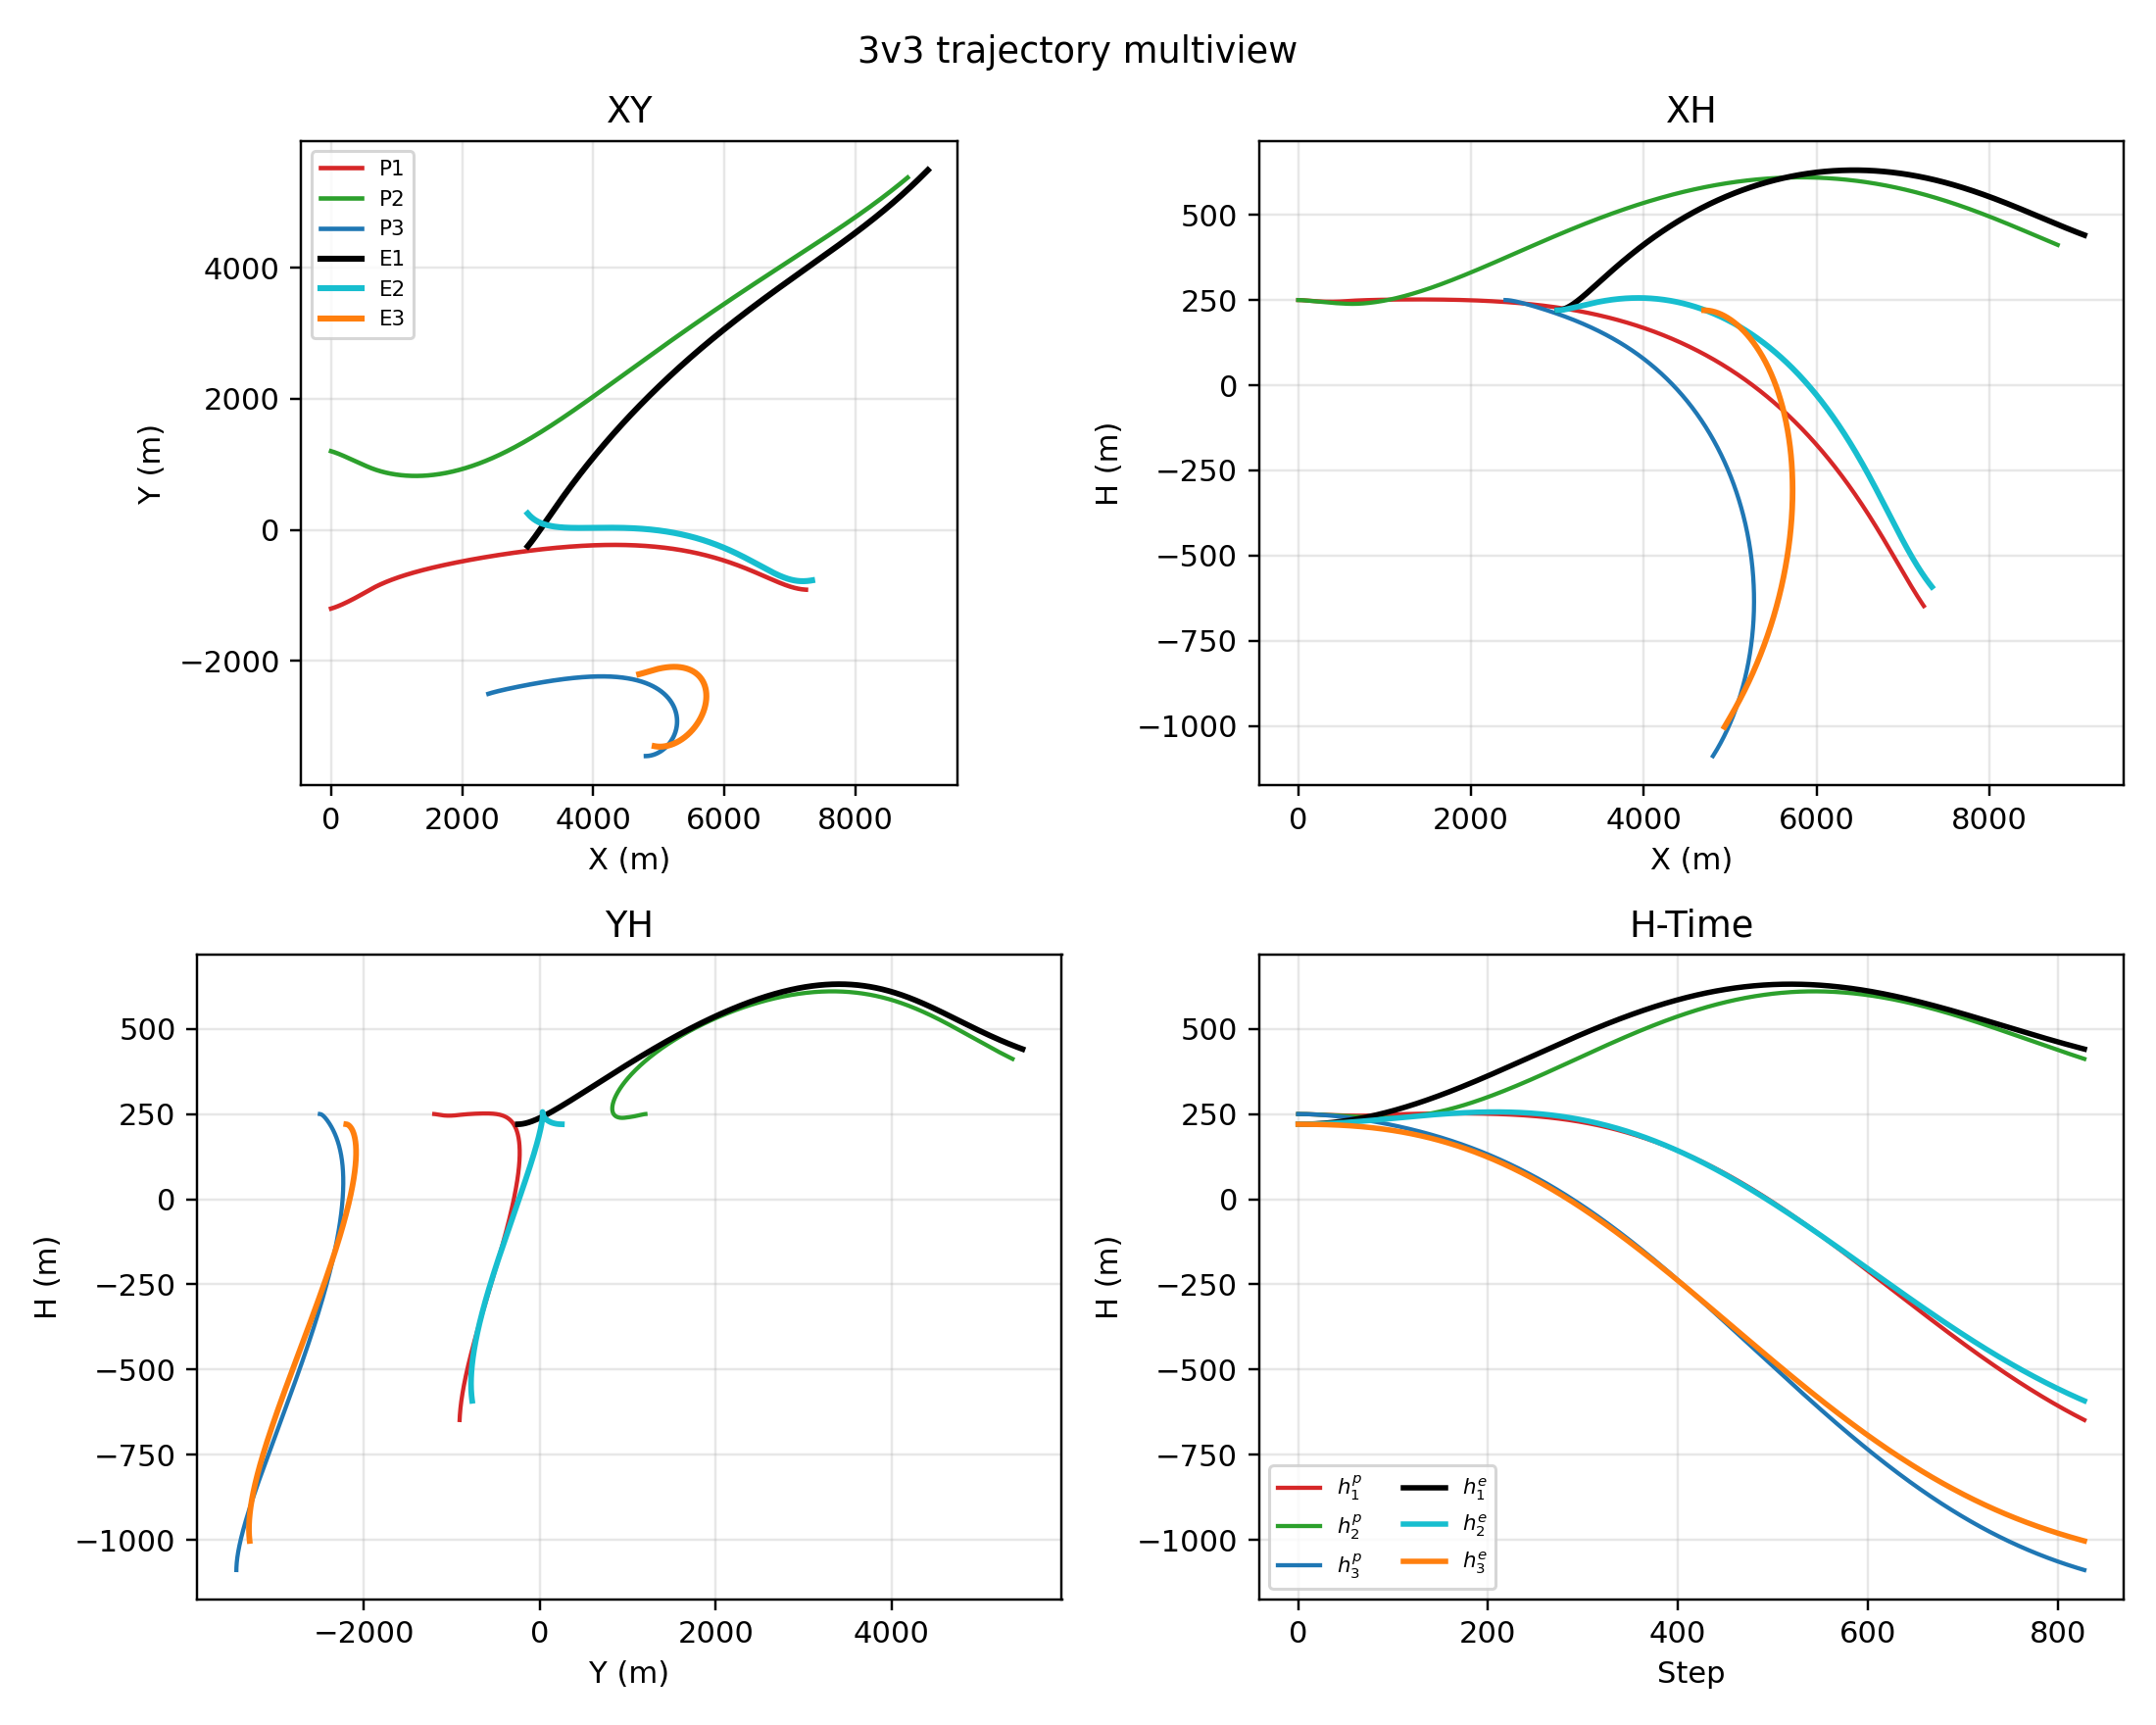
\includegraphics[width=0.48\linewidth]{figs/3v3_traj_main.png}}\hfill
    \subfloat[Old-target vs. new-target errors]{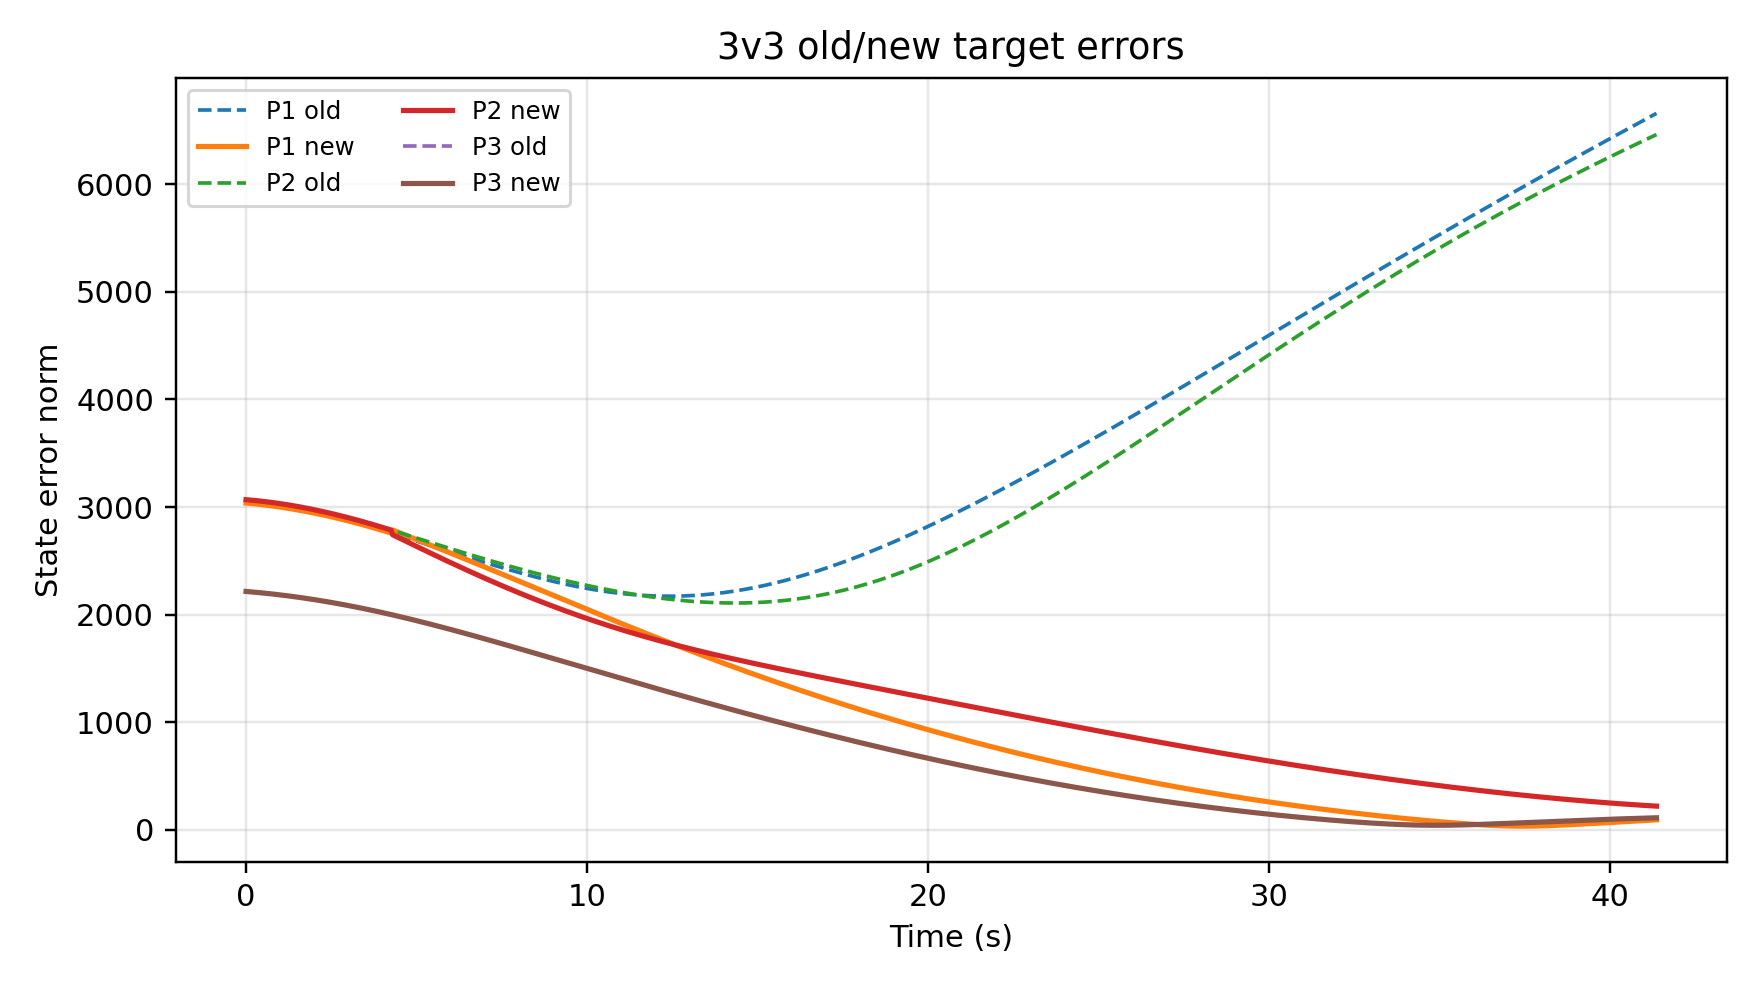
\includegraphics[width=0.48\linewidth]{figs/3v3_oldnew_main.png}}
    \caption{Main 3v3 evidence from Run A. A natural switch occurs when the new assignment produces a smaller local residual cost.}
    \label{fig:3v3_main}
\end{figure}

\begin{figure}[t]
    \centering
    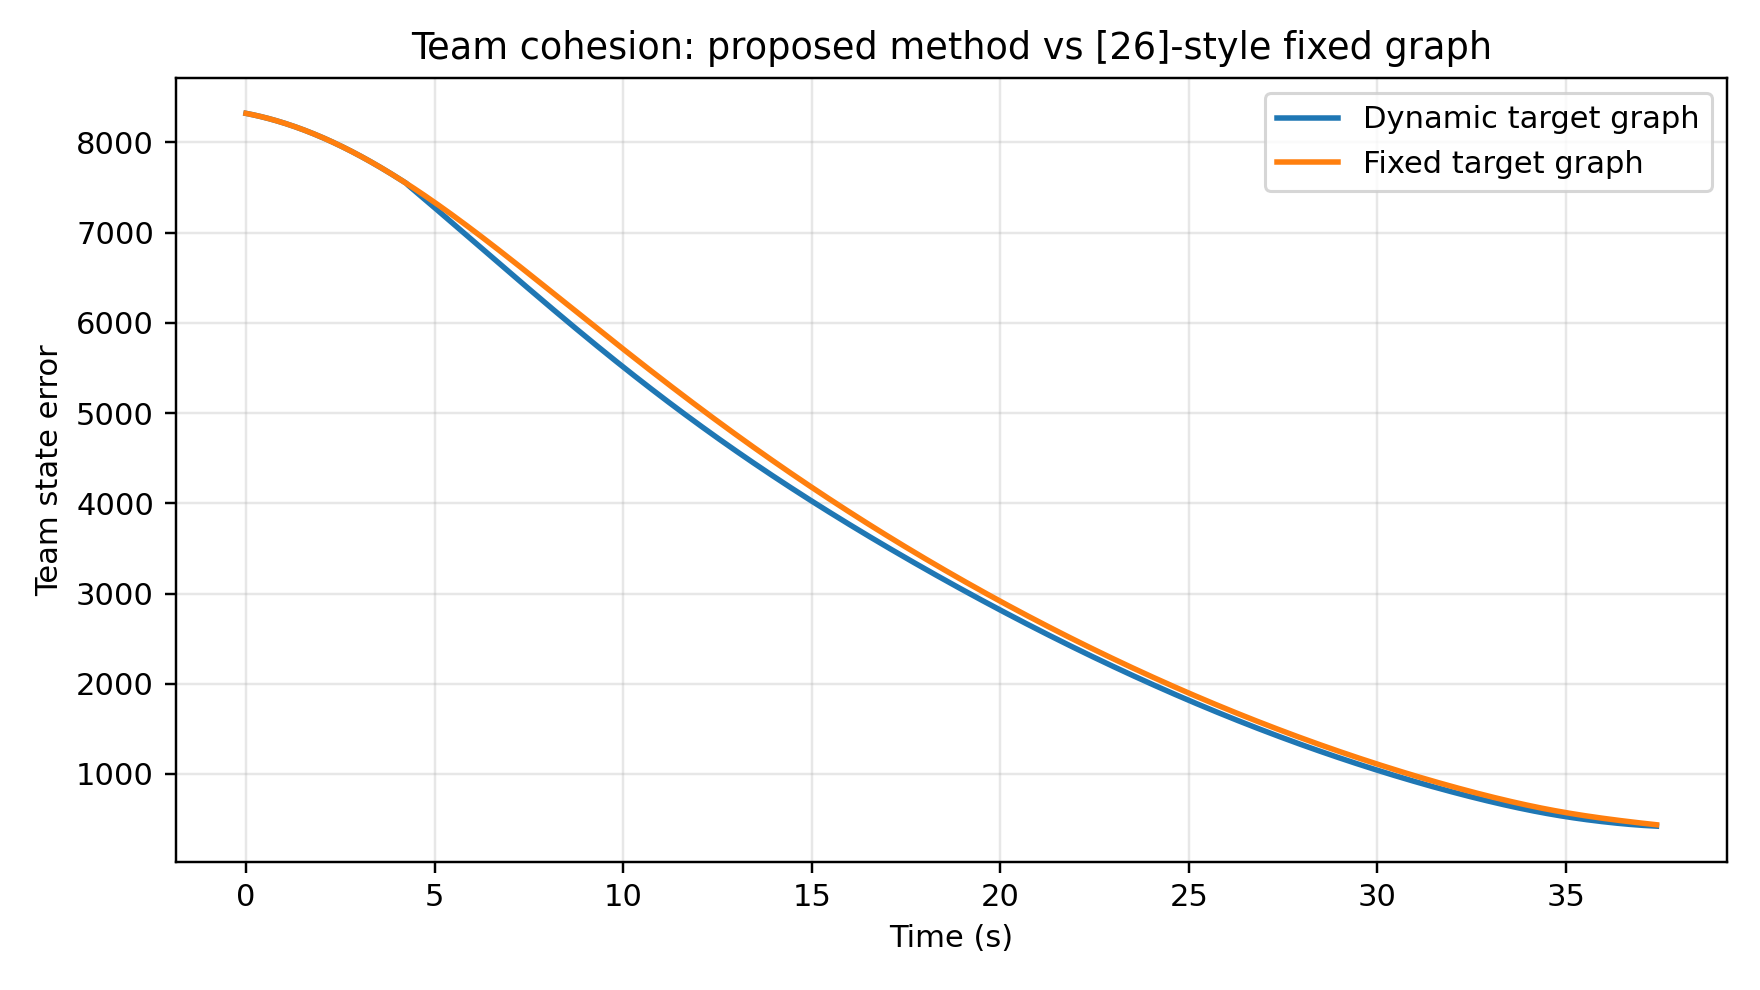
\includegraphics[width=0.88\linewidth]{figs/3v3_team_main.png}
    \caption{3v3 team-error comparison in Run A. The dynamic graph achieves a smaller final team error than the fixed-graph baseline.}
    \label{fig:3v3_team}
\end{figure}

\subsection{5v3: Generalized $m$-vs.-$n$ Extension}
The 5v3 case is used to demonstrate that the same framework extends beyond the standard benchmark scale. Fig.~\ref{fig:5v3_main} shows the trajectory and team-error comparison. The generalized setting preserves the same core ingredients as the smaller cases: nonlinear agent dynamics, bounded-input value-function control, and dynamic graph reassignment. No additional case-specific controller redesign is introduced.

In this generalized run, the dynamic graph reduces capture time from 38.45~s to 31.85~s and lowers mean assigned error from 400.965 to 358.701. The final maximum assigned error is 83.638. The switch timeline records one switch at the initial stage, which is enough to improve the transient pursuit allocation. Compared with the 3v3 benchmark, the 5v3 results show that the same graph-update logic remains effective when the pursuer team becomes larger than the number of evaders.

\begin{figure}[t]
    \centering
    \subfloat[5v3 trajectory]{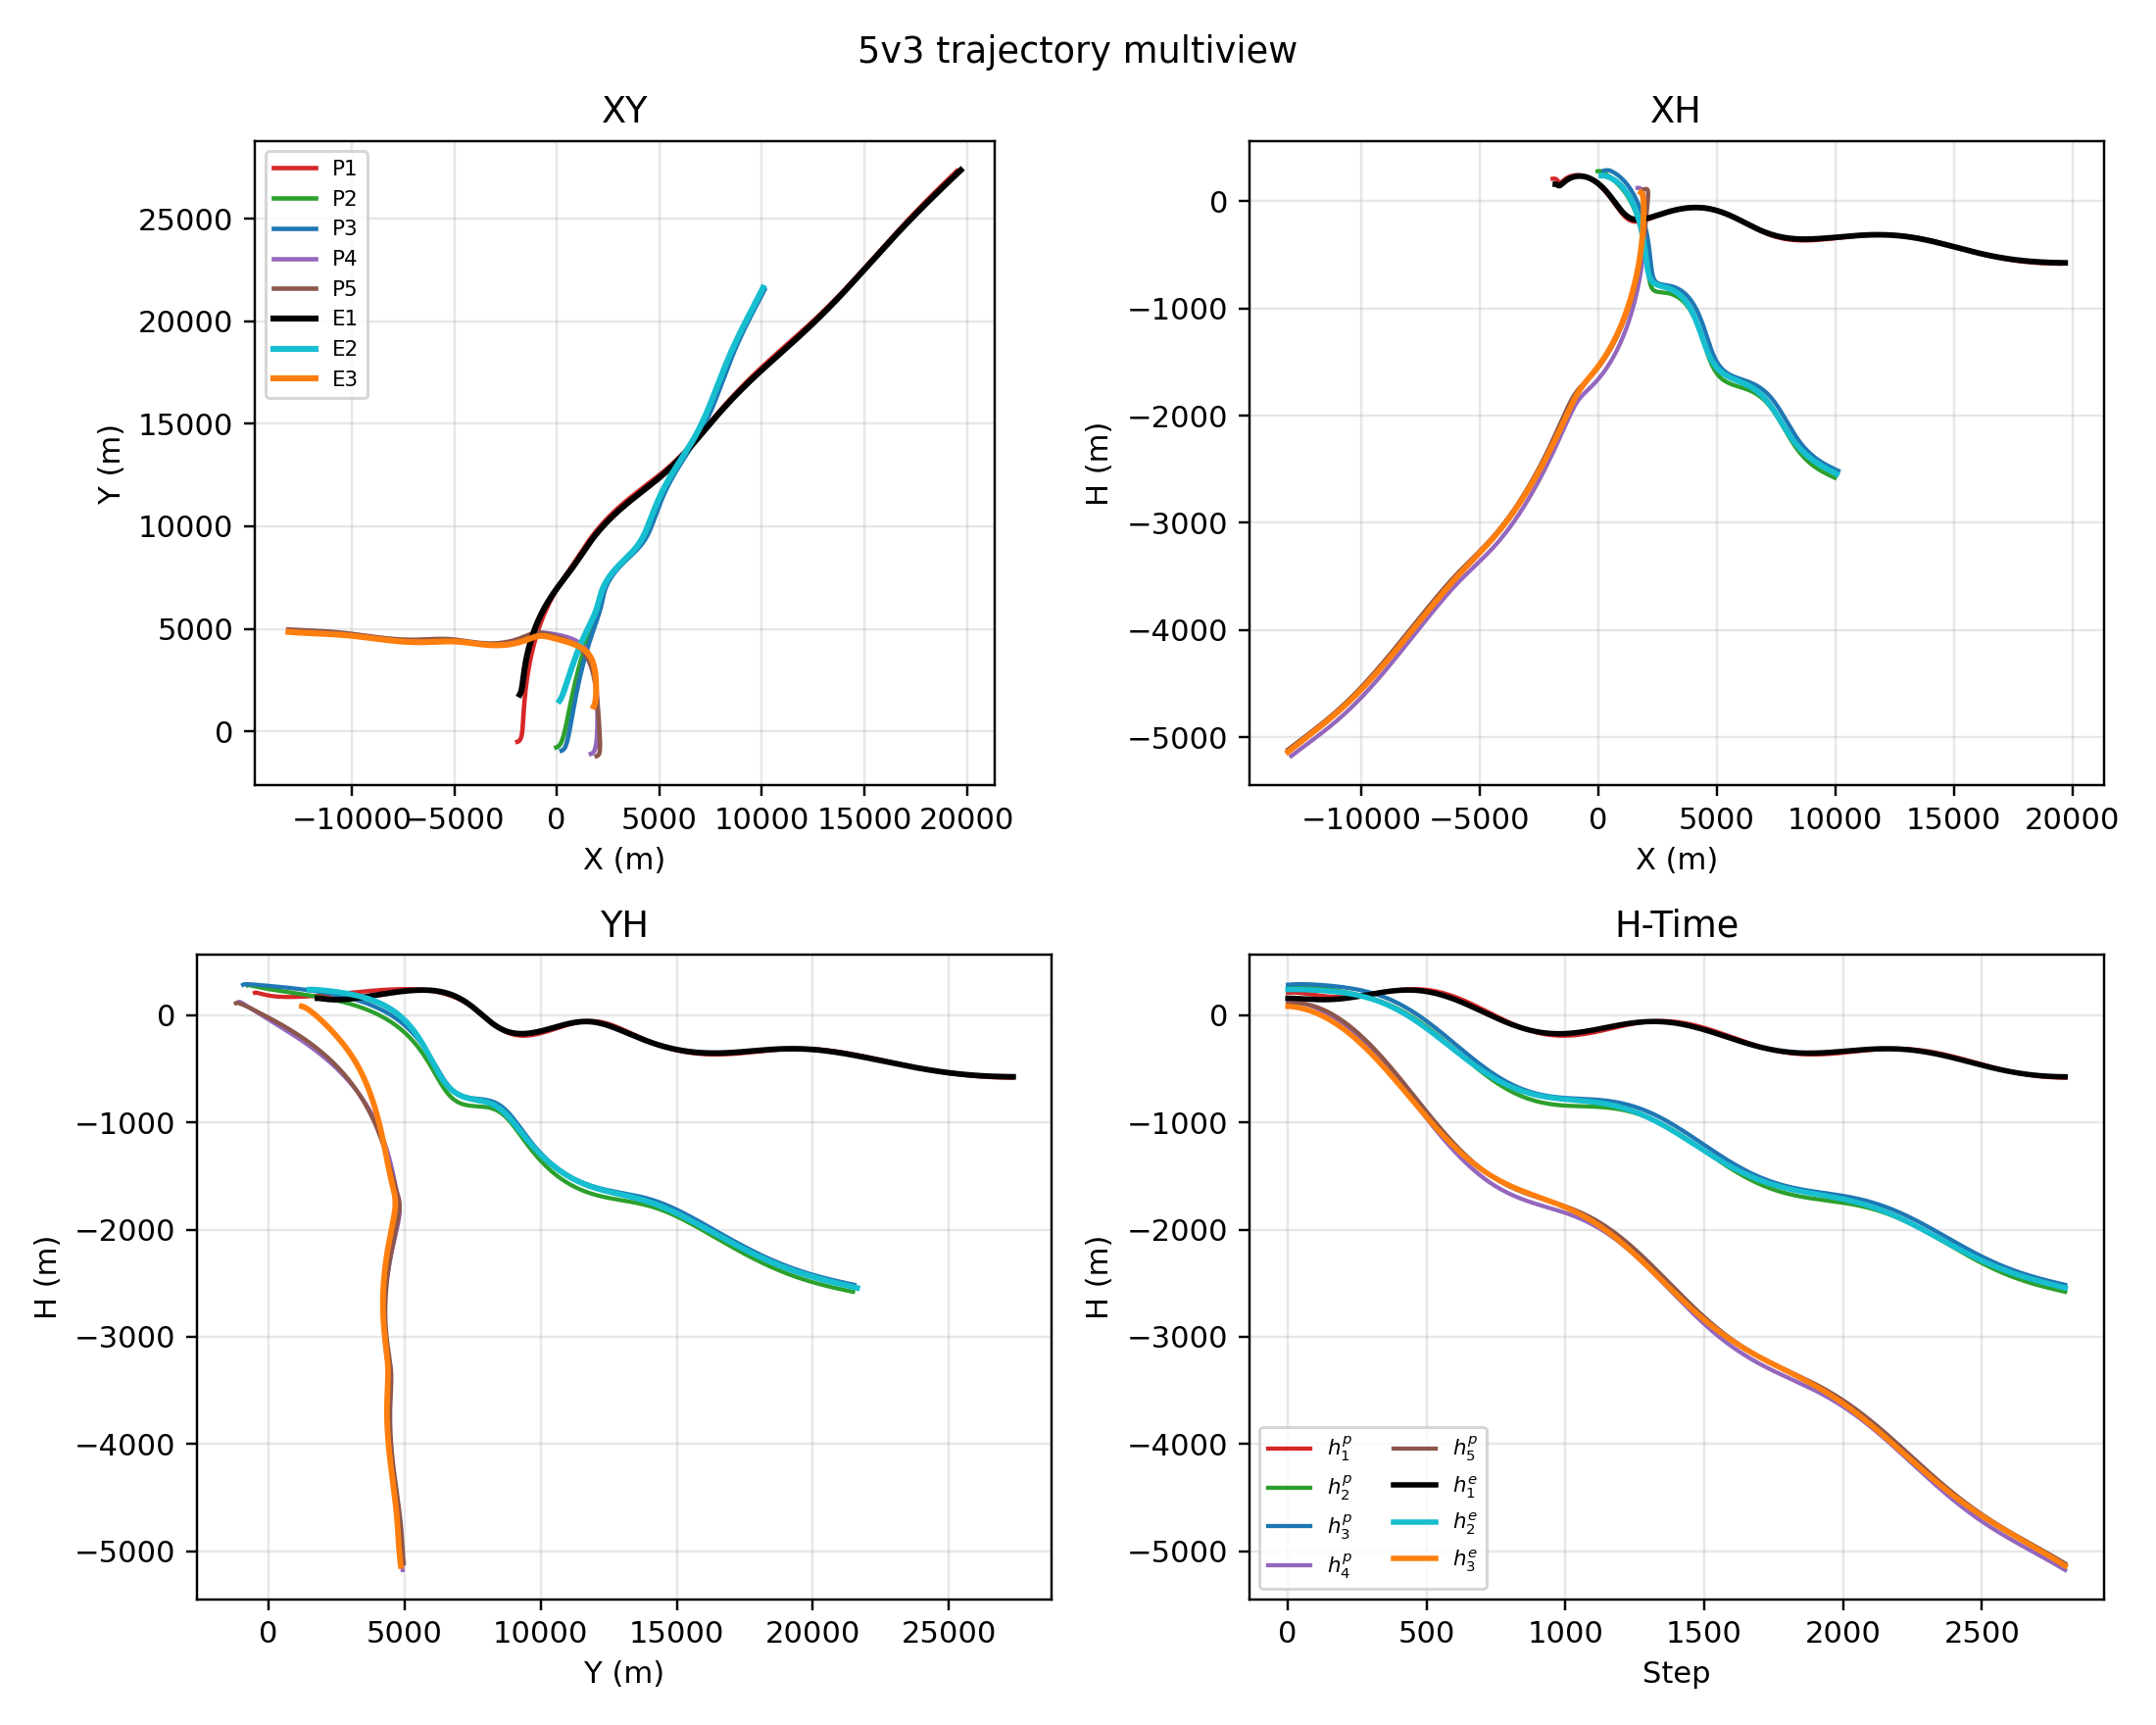
\includegraphics[width=0.48\linewidth]{figs/5v3_traj_main.png}}\hfill
    \subfloat[5v3 dynamic-vs.-fixed team error]{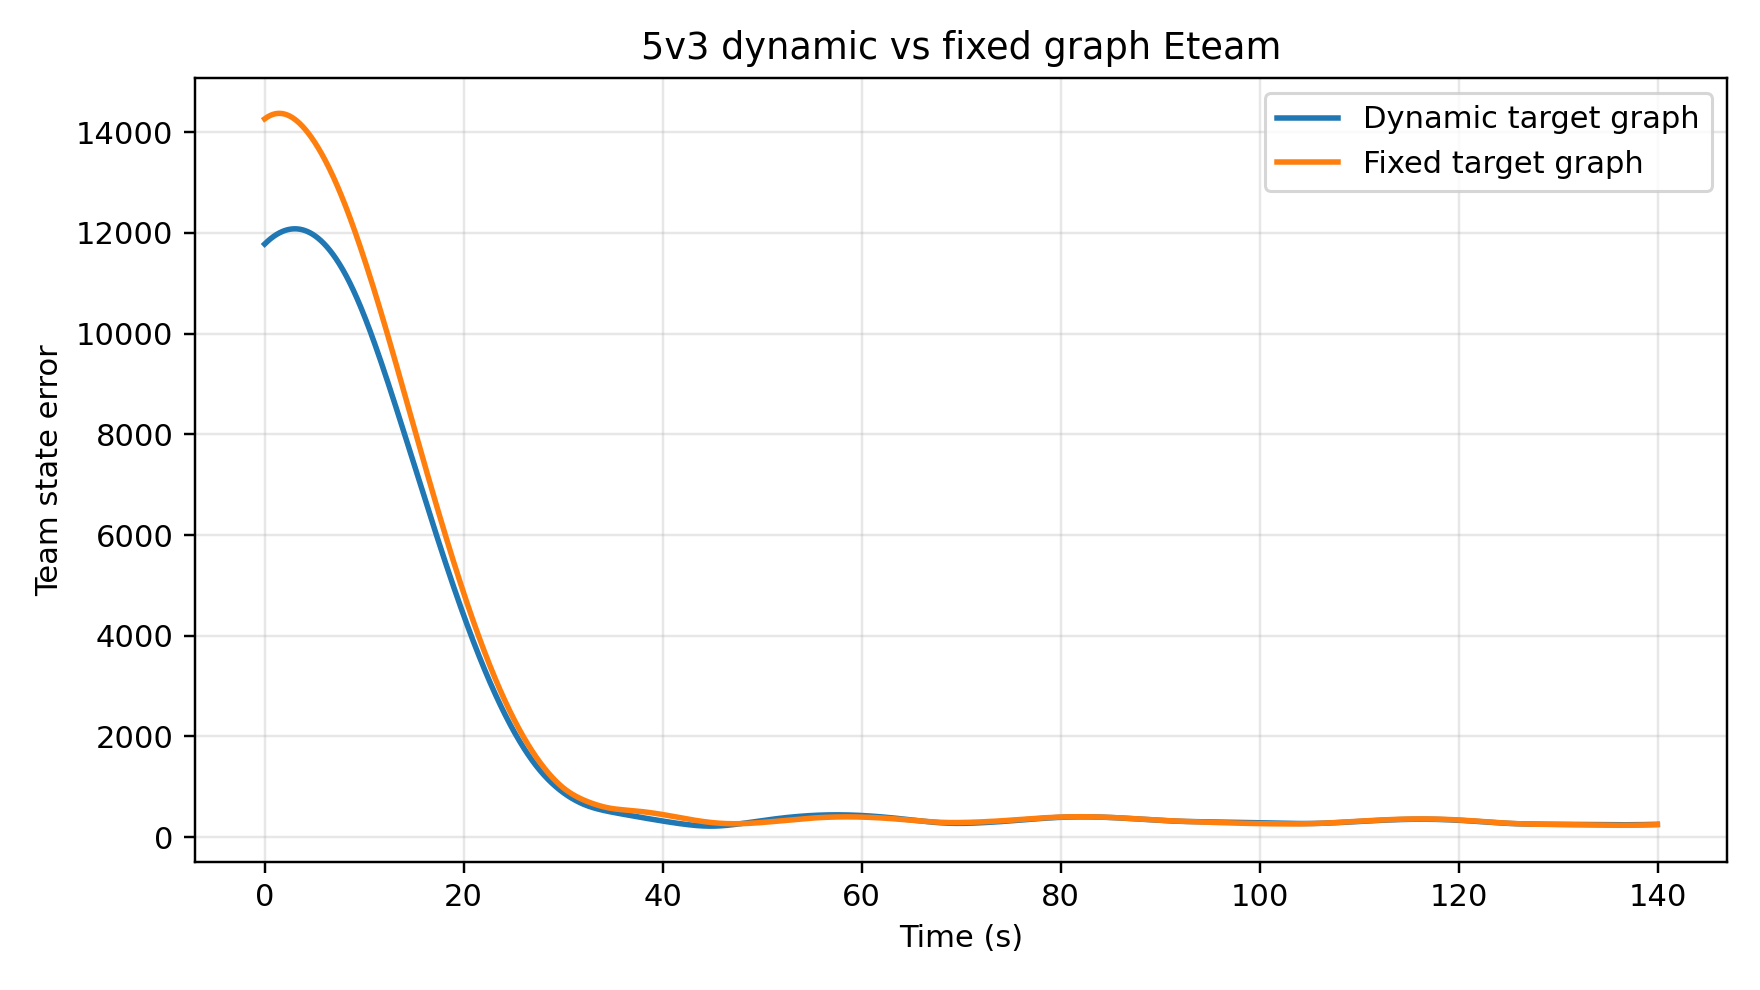
\includegraphics[width=0.48\linewidth]{figs/5v3_team_main.png}}
    \caption{Generalized 5v3 validation. The same bounded-input control and dynamic-graph mechanism remain effective after increasing the team size.}
    \label{fig:5v3_main}
\end{figure}

Table~\ref{tab:main_results} summarizes the main results from Run A, Run B, and the generalized 5v3 case.

\begin{table}[t]
\caption{Main numerical results used in the paper.}
\label{tab:main_results}
\centering
\small
\begin{tabular}{lcccc}
\toprule
Case & Capture time (s) & Final $E_{\text{team}}$ & Mean err. & Notes \\
\midrule
3v1 Run A & 29.95 & 382.820 & -- & Final max err. 158.822 \\
3v1 Run B & 29.95 & 382.820 & -- & Final max err. 158.822 \\
3v3 Run A dyn. & -- & 423.921 & -- & 1 switch at 4.3~s \\
3v3 Run A fixed & -- & 437.024 & -- & Same weights/seed \\
3v3 Run B dyn. & -- & 505.874 & -- & 1 switch at 4.0~s \\
3v3 Run B fixed & -- & 457.870 & -- & Same weights/seed \\
5v3 dyn. & 31.85 & 256.707 & 358.701 & 1 switch at 0.0~s \\
5v3 fixed & 38.45 & 248.990 & 400.965 & Same weights/seed \\
\bottomrule
\end{tabular}
\end{table}

\subsection{Runtime and Network Efficiency}
In addition to control performance, the implementation also records runtime and critic-network counts. The original benchmark-style runs report three critics for both 3v1 and 3v3, while the estimated number of conventional actor-critic networks is twelve, yielding a 75\% reduction in network count. For the generalized 5v3 case, the system uses five critics and an estimated sixteen actor-critic networks, corresponding to a 68.75\% reduction.

The generalized runner also records the average runtime per simulation step. In the 5v3 case, the total runtime is 7.1968~ms/step, with 7.1230~ms/step in training and 7.6323~ms/step in dynamic-graph evaluation. In the full generalized batch, the parallel runner achieves an estimated speedup of approximately 1.23$\times$ with two worker processes. These measurements show that the framework is not only behaviorally effective, but also suitable for repeated multi-case validation.

\begin{table}[t]
\caption{Network and runtime statistics.}
\label{tab:runtime}
\centering
\small
\begin{tabular}{lccc}
\toprule
Case & Critics & AC est. nets & Runtime \\
\midrule
3v1 & 3 & 12 & -- \\
3v3 & 3 & 12 & -- \\
5v3 & 5 & 16 & 7.1968 ms/step \\
Batch (2 workers) & -- & -- & 1.23$\times$ speedup \\
\bottomrule
\end{tabular}
\end{table}

\section{Conclusion}
This paper presented a generalized implementation framework for nonlinear bounded-input multi-agent pursuit-evasion games. The framework combines six-state nonlinear aircraft dynamics, value-function-based saturated control, dynamic target reassignment, and generalized $m$-vs.-$n$ scenario generation under a common interface. Three levels of evidence were provided. The 3v1 case verified stable nonlinear pursuit, assigned-error decay, bounded control input, critic convergence, and saturation sensitivity. The 3v3 case verified that dynamic target reassignment can naturally occur and improve team-error performance under the same trained weights and identical evaluation conditions. The 5v3 case showed that the same implementation extends to a larger generalized setting and improves capture time and mean assigned error relative to a fixed-graph baseline. These results indicate that the proposed system is effective for both standard benchmark verification and scalable $m$-vs.-$n$ pursuit-evasion simulation.

\bibliographystyle{IEEEtran}
\bibliography{refs}

\end{document}
